\documentclass{article}

\usepackage[portuguese]{babel}

\usepackage{amsmath}
\usepackage{graphicx}
\usepackage{empheq}
\usepackage[hidelinks]{hyperref}

\title{P1}
\date{}
\author{Ryuji}

\begin{document}
\section{Projeto}
\paragraph{} Projetar um toco de microfita para 1GHz baseado no exercicio da aula 5.

\begin{figure}[h!]
	\begin{center}
	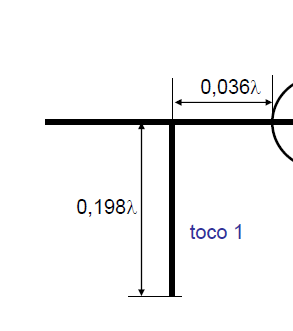
\includegraphics[width=200px]{images/img_proj.png}
	\end{center}
	\caption{Circuito}
	\label{fig:imagem1}
\end{figure}

\paragraph{}Considerar uma carga de $5 + j3,5$ $\Omega$

\begin{figure}[h!]
	\begin{center}
	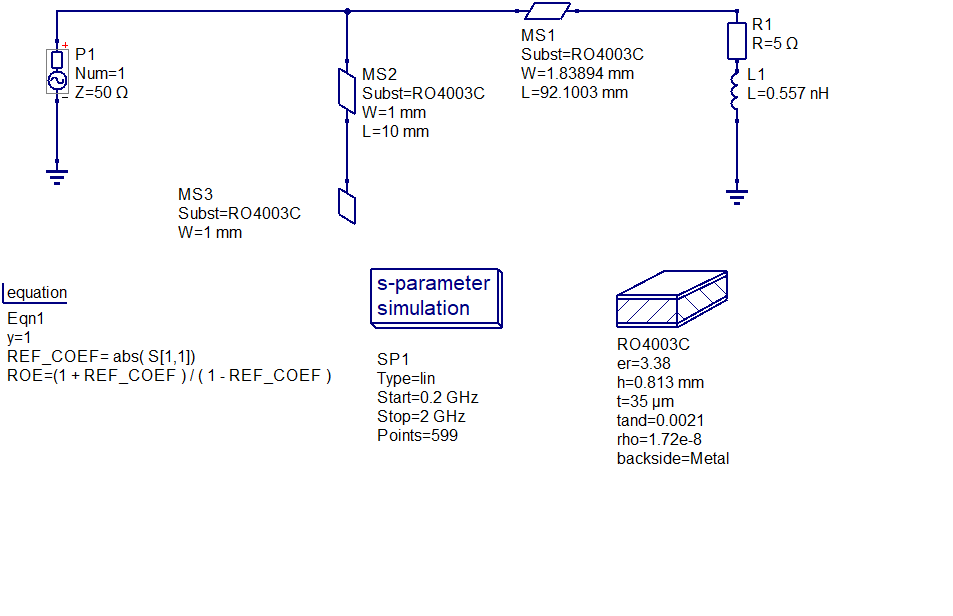
\includegraphics[width=\linewidth]{images/diagrama_ini.png}
	\end{center}
	\caption{Diagrama disponibilizado}
	\label{fig:imagem1}
\end{figure}

\section{Determinando o $L$}

\paragraph{} Como as medidas já foram dadas, e $\lambda = 360 graus$, então:

\paragraph{} Para $0,036\lambda = 12,96 graus$:

\begin{figure}[h!]
	\begin{center}
	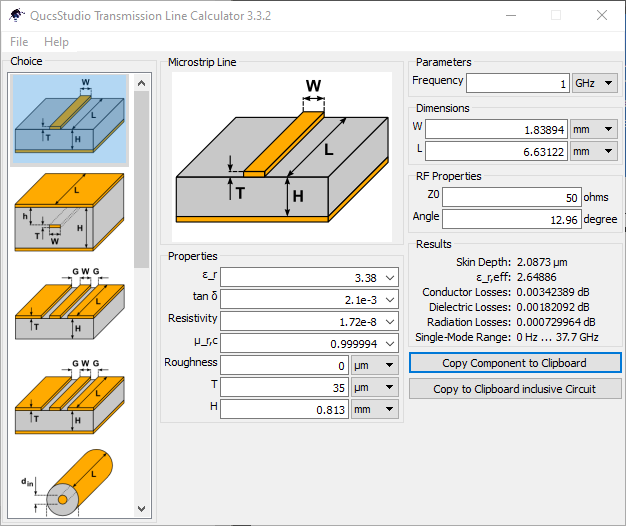
\includegraphics[width=200px]{images/calculadora_1.png}
	\end{center}
	\caption{Calculadora QucsStudio}
	\label{fig:imagem1}
\end{figure}

\paragraph{} Para $0,198\lambda = 71,28 graus$:

\begin{figure}[h!]
	\begin{center}
	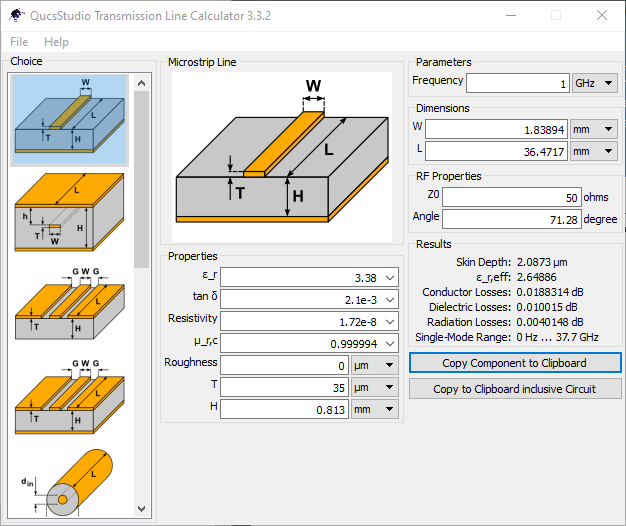
\includegraphics[width=200px]{images/calculadora_2.png}
	\end{center}
	\caption{Calculadora QucsStudio}
	\label{fig:imagem1}
\end{figure}

\paragraph{} Colocando os valores no diagrama:

\begin{figure}[h!]
	\begin{center}
	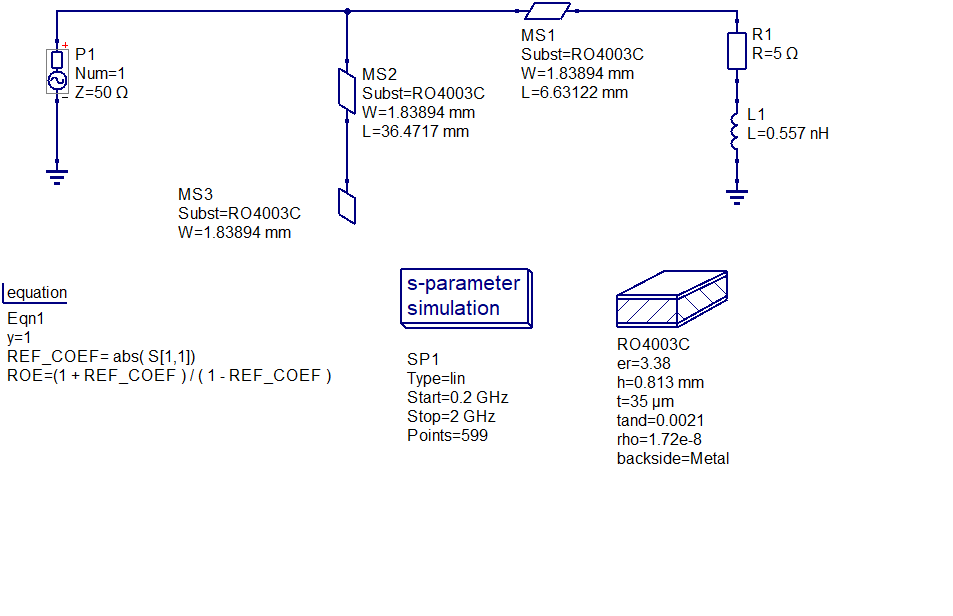
\includegraphics[width=\linewidth]{images/diagrama_fin.png}
	\end{center}
	\caption{Diagrama final}
	\label{fig:imagem1}
\end{figure}

\section{Simulação}

\begin{figure}[h!]
	\begin{center}
	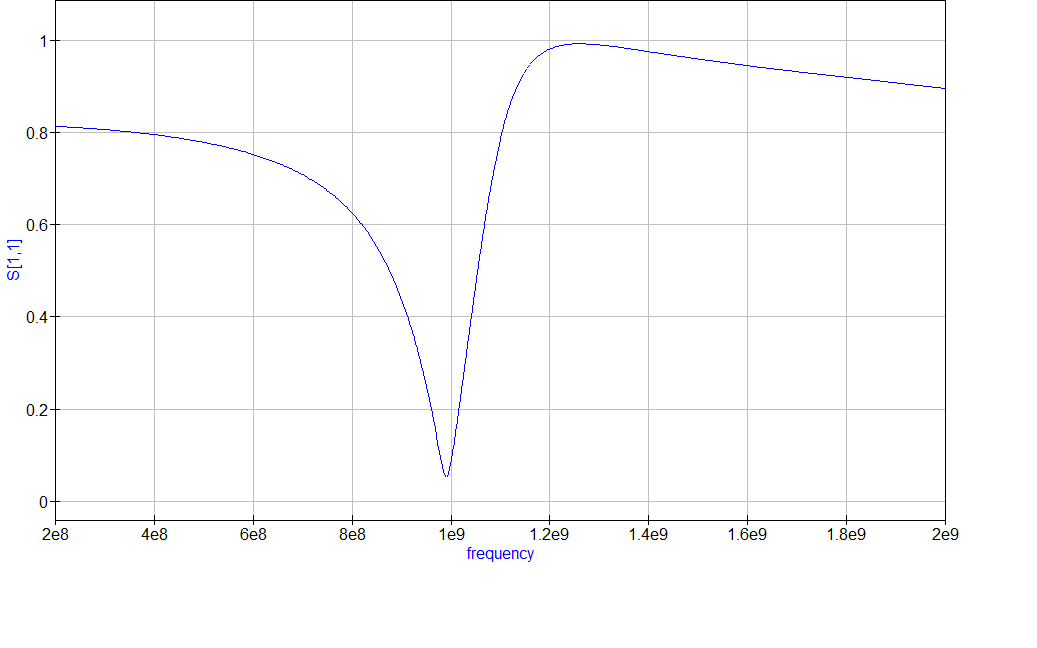
\includegraphics[width=\linewidth]{images/sim_resposta.png}
	\end{center}
	\caption{Parametro S[1, 1]}
	\label{fig:imagem1}
\end{figure}

\begin{figure}[h!]
	\begin{center}
	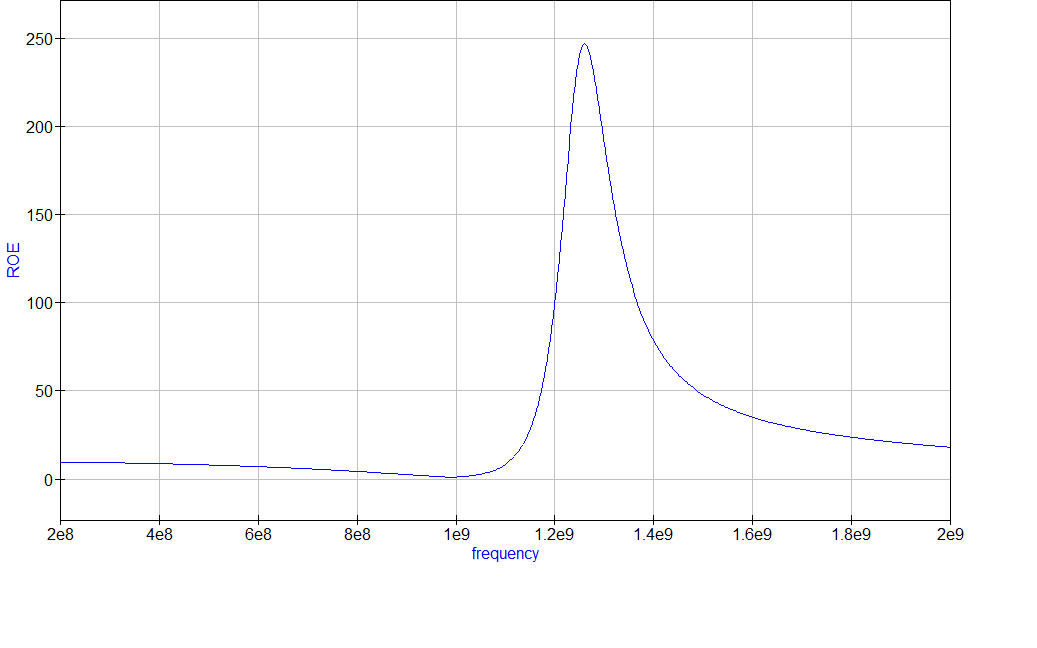
\includegraphics[width=\linewidth]{images/sim_roe.png}
	\end{center}
	\caption{ROE}
	\label{fig:imagem1}
\end{figure}

\end{document}